\def\QRCODE{tp_en_attente_TUT.IMG.tomography_matlabqrcode.png}
\def\QRPAGE{http://www.iptutorials.science/tree/master/tp_en_attente/TUT.IMG.tomography/matlab}
\mcorrectionsection{MATLAB correction}


\subsection{Acquisition simulation}

The MATLAB built-in function is used to generate a phantom image.

\begin{matlab}
% phantom image generation
I = phantom();

%% Projection with an angular step of 1 degree 
angle = 1;
theta = 0:angle:180;
S=simuProjection(I, theta);
imshow(S, []);
\end{matlab}

The simulation of the projection is simply an addition of all gray-levels of the pixels, after rotating the image in order to simulate the rotation of the object (or of the sensor).
\iflabelexists{fig:tomography:enonce:contri}{See Fig.\ref{fig:tomography:enonce:contri}}{See Fig.\ref{fig:tomography:matlab:contri}.

\begin{figure}[htbp]
 \centering
 
\includegraphics[width=.4\linewidth]{contri.png}
 \caption{Simulation of the projection: contribution of a line $D$ before rotation.}
 \label{fig:tomography:matlab:contri}
\end{figure}
}

\begin{matlab}
function S=simuProjection(I, theta)
% simulation of the generation of a sinogram
% I : original image (phantom for example)
% theta: angles of projection
taille=size(I);
S=zeros(taille(2),length(theta));

for i=1:length(theta)-1,
    image1=imrotate(I, theta(i), 'bilinear', 'crop');
  
    S(:,i)=sum(image1');
end
\end{matlab}


\subsection{Backprojection algorithm}
The backprojection algorithm will sum-up all the contributions of each projection.

\begin{matlab}
function R=backprojection(P, theta, filtre)
% Backprojection of a projected image P,
% at all angles 'theta'
% filtre: bool, applies filtering if True
N = size(P,1);
R =zeros(N);

% in case of filtered back-projection
h = RamLak(31);

% loops over all angles
for i=1:length(theta),
    proj = P(:,i);
    
    % filtered back-projection
    if filtre==1
        proj = conv(proj, h, 'same');
    end
    
    proj2 = repmat(proj, 1, N);
    proj2 = imrotate(proj2, -theta(i), 'bilinear', 'crop');
    
    R = R + proj2;
end 
\end{matlab}

The results is better in the case of a filtered backprojection. The RamLak function is provided and illustrated in Fig.\ref{fig:tomography:matlab:ramlak}.
\begin{matlab}
function [ramlak] = RamLak(width)
% Ramlak filter of size width
% width must be odd
k=-width:1:width;

for indice = 1:length(k);
  if(k(indice)==0) % valeur du centre
     ramlak(indice)=pi/4;
  elseif(mod(k(indice),2)==1) % indices pairs
     ramlak(indice)=-1/(pi*k(indice)^2);
  else % indices impairs
     ramlak(indice)=0;
  end
end 
\end{matlab}

\begin{figure}[htbp]
 \centering
 
 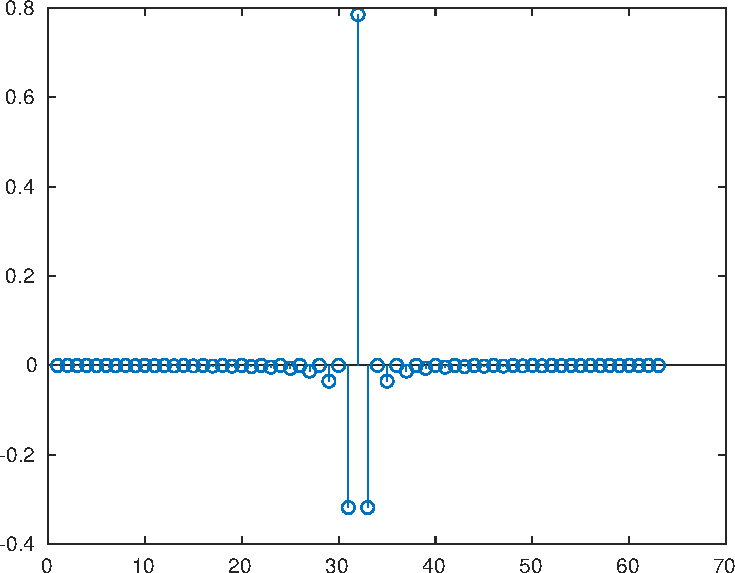
\includegraphics[width=.45\linewidth]{ramlak.pdf}
 
 \caption{RamLak function.}
 \label{fig:tomography:matlab:ramlak}
\end{figure}

The reconstruction of the original image is obtained by the following code:
\begin{matlab}
%% reconstruction: simple back-projection
R1=backprojection(S, theta, 0);

imshow(R1, []);

%% Filtered back-projection
R2=backprojection(S, theta, 1);
imshow(R2, []);

%% \matlabregistered{} built-in functions
s=radon(I, theta);
imshow(s, []);

r=iradon(s, theta);
figure();
imshow(r, []); 
\end{matlab}

\begin{figure}[htbp]
 \centering
 
 \subfloat[Original phantom image.]{
\includegraphics[width=.3\linewidth]{phantom.png}}\hfill
  \subfloat[Unfiltered backprojection.]{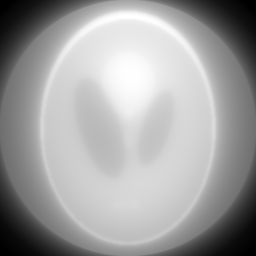
\includegraphics[width=.3\linewidth]{unfiltered_backprojection.png}}\hfill
 \subfloat[Filtered backprojection.]{
\includegraphics[width=.3\linewidth]{filtered_backprojection.png}}
 \caption{Reconstruction by backprojection.}
 \label{fig:tomography:matlab:backprojection}
\end{figure}

